\documentclass{bioinfo}
\usepackage{url}

\usepackage[british,english]{babel}
\usepackage{mathpazo}
\usepackage[T1]{fontenc}
% \usepackage[latin9]{inputenc}
\usepackage{float}
\usepackage{amsmath}
\usepackage{graphicx}
\usepackage{setspace}
\usepackage{amssymb}
\usepackage{natbib}
\usepackage[title]{appendix}
\usepackage{siunitx}
\usepackage{chngcntr}
\usepackage{algorithmic}
\renewcommand{\algorithmicrequire}{\textbf{Input:}}
\renewcommand{\algorithmicensure}{\textbf{Output:}}

\makeatletter
\newfloat{algorithm}{H}{loa}[section]
\floatname{algorithm}{Algorithm}
\counterwithout{algorithm}{algorithm}
\def\argmin{\mathop{\operator@font arg\,min}} 
\def\argmax{\mathop{\operator@font arg\,max}} 
\makeatother

\copyrightyear{}
\pubyear{}

\begin{document}
\firstpage{1}

\title[QuickBundles]{QuickBundles, a method for tractography simplification}

\author[Garyfallidis, Brett, Correia, Williams and
Nimmo-Smith]{Eleftherios~Garyfallidis\,$^{1,3,*}$, Matthew~Brett\,$^{2}$,
  Marta~Morgado~Correia\,$^{3}$, Guy~B.~Williams\,$^{4}$ and
  Ian~Nimmo-Smith\,$^{3}$\footnote{to whom correspondence should be
    addressed. e-mail: garyfallidis@gmail.com}}

\address{\,$^{1}$Wolfson College, University of Cambridge, Cambridge, UK\\
  \,$^{2}$University of California, Henry H. Wheeler, Jr. Brain Imaging Center, Berkeley, CA.\\
  \,$^{3}$MRC Cognition and Brain Sciences Unit, Cambridge, UK.\\
  \,$^{4}$Wolfson Brain Imaging Centre, University of Cambridge,
  Cambridge, UK.}


\history{}

\editor{}

\maketitle

\begin{abstract}
\noindent
Diffusion MR datasets produce large numbers of streamlines which
are hard to visualize, interact with, and interpret in a clinically
acceptable time scale, despite numerous proposed approaches. As a
solution we present a simple, compact, tailor-made clustering algorithm,
QuickBundles (QB), that overcomes the complexity of these large data
sets and provides informative clusters in seconds. Each QB cluster can
be represented by a single centroid streamline; collectively these
centroid streamlines can be taken as an effective representation of the
tractography. We provide a number of tests to show how the QB reduction
has good consistency and robustness. We show how the QB reduction can
help in the search for similarities across several subjects.

\section{Keywords:} Tractography, Diffusion MRI, Fiber clustering, White
matter Segmentation, Dimensionality Reduction, Clustering algorithms, DTI.

\end{abstract}


\section{Introduction}

Following the acquisition of diffusion MR scans, processes of
reconstruction and integration are performed to create a tractography: a
dataset composed of streamlines, which are sequences of points in 3D
space. Irrespective of the types of reconstruction and integration, a
tractography can contain a very large number of streamlines (up to
$10^6$) depending principally on the number of seed points used to
generate the tractography but also on how the tractography propagation 
algorithm handles voxels with underlying fiber crossings.

\begin{figure*}[htp]
\centerline{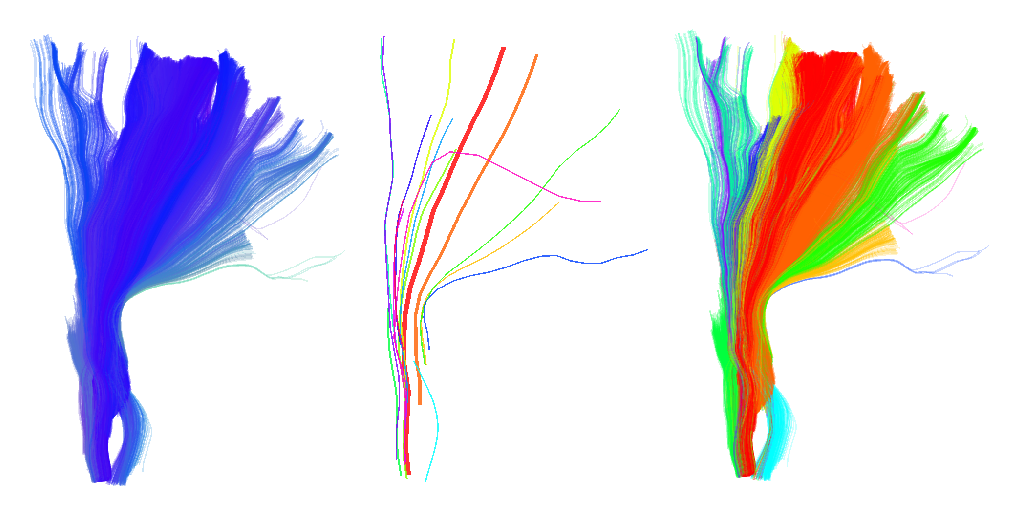
\includegraphics[width=160mm]{Figures/Fig_4_cst_simplification_relabeled_triple.eps}}
\caption{Part of the CST bundle (left in blue) consisting of \num{11041}
  streamlines. At first glance it looks as though all streamlines have a
  similar shape, and possibly converge towards the bottom, and fan out
  towards the top. However, this is a misreading caused by the opaque
  density when all the streamlines are visualised.  QB can help us see
  the finer structure of the bundle and identify its elements. In the
  middle we see the 16 QB centroid streamlines of the CST. We can now
  clearly observe that several parts which looked homogeneous are
  actually broken bundles or bundles with rather different shapes. On
  the right panel we see the streamlines coloured according to their
  cluster label. The distance threshold used here was
  $10$~mm. \label{Flo:cst_pbc}}
\end{figure*}


The size of these tractographies makes them difficult to interpret and
visualize. A clustering of some kind seems to be an obvious route to
simplify the complexity of these datasets and provide a useful
segmentation. As a result, during the last 10 years there have been
numerous efforts by many researchers to address both unsupervised and
supervised learning problems of brain tractography.  As far as we know
all these methods suffer from low time efficiency, i.e.~they are very
slow when used in practice.

%------------------------------------------------------------------------------

In tractography literature we can find approaches which use unsupervised
and/or supervised learning algorithms to create bundles i.e. groupings
of streamlines with similar spatial and shape characteristics. In
supervised learning the datasets are divided into a training and a test
set. For the training set experts will have provided anatomical
labels for a set of manually segmented streamline bundles. Those bundles
will now correspond to tracts e.g.~the corticospinal tract or the
arcuate fasciculus. The task then will be to identify similar
structures amongst the unlabeled streamlines in the test set.

In unsupervised learning the focus is on creating a partitioning of the
streamlines without knowing any labels. In this work we used
unsupervised learning to reduce in an simple and efficient way the
number of streamlines and make manual segmentation of bundles and
tractography exploration a less time consuming task.

We believe that a complete unsupervised method cannot directly create
anatomically valid bundles without extensive prior information
preferably from experts or atlases. This is because anatomical bundles differ considerably both in lengths and in shape
(see \citet{schmahmann2009fiber}) and there is not a single threshold which can cluster a full dataset with anatomical
correspondence (see \citet{Guevara2010}). Furthermore, if one uses such extensive priors then it will be more suitable to use supervised learning
algorithms. Therefore, we propose that unsupervised learning should be
used primarily for dimensionality reduction or simplification of these
large datasets. This is also the focus of the approach that we propose
here.

Most clustering (unsupervised learning algorithms) are in the best case
of complexity $\mathcal{O}(N^2)$ where $N$ the total number of
streamlines: they require the calculation of all pairwise distances between streamlines in order to create a distance matrix. We
  found that most authors tried to create these distance matrices as input to  hierarchical clustering (see \citet{
  moberts2005evaluation, zhang2005dti, Tsai2007, zhang2008identifying, jianu2009exploring, Visser2010, Guevara2010,
  Guevara12}) or spectral clustering
(see \citet{ODonnell_IEEETMI07, o2009tract, jonasson2005fiber,
  ziyan2009consistency}) or affinity propagation (see
\citet{leemans17new, malcolm2009filtered}). However, they had to restict
themselves to only a subset of the complete dataset because the
calculations were heavy and the distance matrix too big for computers
with standard memory capacity. For example, \citet{ODonnell_IEEETMI07}
used only \num{10000} streamlines (~10\% of the initial tractography)
and \citet{Visser2010} used recombinations of \num{10000} streamlines.
We give here an example of how large that distance matrix can be if used
with a full dataset. Just for \num{100000} streamlines 38 GBytes are
required and for 1 million streamlines 3.6 TBytes of memory are required
(4 bytes floating point precision).

Other clustering methods have also been proposed that use graph
theoretic approaches (see \citet{brun2004clustering, gerig2004analysis, ElKouby2005}),
k-nearest neighbours (see \citet{Ding2003a, moberts2005evaluation}),
gaussian processes (see \citet{wassermann2010unsupervised}),
hierarchical dirichlet processes (see \citet{wang2010tractography}),
currents (see \citet{Durrleman2009, durrleman2010registration}),
adaptive mean shift (see \citet{zvitia2008adaptive, Zvitia2010}),
k-means (see \citet{ElKouby2005}) and expectation maximization (see
\citet{Maddah_IEEEBI2008}). These methods although often try to avoid distance matrices they still suffer from low time
efficiency. All the same, if clustering is to be used in clinical practice or to make neuroscientists' analysis more efficient and practical we need
algorithms that can provide useful clusters and cluster descriptors in
acceptable time. None of the papers covered in this literature review
provide a solution for this issue of efficiency and most of the methods
would require from many hours to many days to run on a standard sized
dataset.

%Distances
%\citet{zhang2003visualizing, corouge2004towards, Corouge2004, Corouge2006}
%me and Visser

%Representation
%Discretization \citet{EGMB10}, \citet{Visser2010}
%B-splines \citet{Maddah_MICCA2005}  
%quintic B-splines \citet{maddah2006statistical}   
%Fourier descriptors



%Most authors agree that unsupervised learning with tractographies is a
%difficult problem as the datasets are very large, dense, cluttered with
%noisy streamlines which could have no anatomic relevance, and the actual
%anatomical bundles are interwoven in a complicated way in several brain
%regions.  We think that in order to find larger anatomical clusters a
%significant amount of anatomical prior knowledge needs to be introduced
%in a way that is not yet established.

%For these reasons we propose to take a step back to first get the
%tractography into a suitable form for working with neuroanatomists to
%capture this prior knowledge. The clustering that we propose
%concentrates on reducing the complexity of the data rather than finding
%bundles with hopefully anatomical relevance. We believe this step is
%more useful at this stage of tractography analysis research.

%Most of these proposed tractography clustering algorithms are very slow
%and many need to calculate a matrix of inter-streamline distances of
%size $\mathcal{O}(N^2)$.  \textbf{Isn't this repetitive?} This number of
%computations puts a very heavy load on clustering algorithms, making
%them hard to use for everyday analysis as it is difficult to compute all
%these distances or store them in memory. For the same reason, no current
%algorithm is practical for real time clustering on a large number of
%streamlines -- despite the innovations in tractography clustering
%algorithms there is no parallel uptake by anatomists or clinicians. The
%heavy computational demands of clustering add a further overhead to the
%use of tractography for clinical applications but also put a barrier on
%understanding and interpreting the quality of diffusion MR
%datasets. Moreover methods described as `automatic' in reality require
%significant intervention using neuroanatomical knowledge. \textbf{In
%  fact isn't all this covered earlier on in this version of the
%  Introduction?}

In fact tractographies have high levels of redundancy with very many
quite similar streamlines. Our approach is to take advantage of this to
reduce the size and dimensionality of the datasets as a precursor for
higher complexity classification and/or input from experts. To address
these key issues of time and space we present a stable, generally linear
time clustering algorithm that can generate meaningful clusters of
streamlines in seconds with minimum memory consumption. Our approach is
 straightforward and we do not need to calculate all pairwise
distances unlike most existing methods. Furthermore we can update our
clustering online. In this way we can overcome the previous barriers of
space and time.

We show that QuickBundles can generate these clusters many times much faster than any other available method, and that it can be used to cluster from a few hundred to many millions of streamlines.

We think that there is no current unsupervised anatomical segmentation method that can have general usability without expert knowledge
integration. Nonetheless, neuroanatomists often disagree on definition
of major structures or on which streamlines correspond to actual tracts
\citep{schmahmann2009fiber, makris2005segmentation,
  frey2008dissociating,catani2005perisylvian, moriBook,
  fernandez2012high, verstynen2011vivo}.  What we propose is to use QuickBundles to simplify the tractography at the level where such
distinctions are not an issue (see Fig.~\ref{Flo:cst_pbc}). On top of these simplifications we can use other methods of
higher complexity much more efficiently.

\begin{methods}

\section{Methods and Materials}

\subsection{\label{sub:track-distances}Streamline distances and
  preprocessing}

A wide range of approaches have been taken in the literature for
representing or coding for tractographies~\citep{Guevara2010,
  chung2010cosine}. The approach we have taken with streamline coding
has gone in parallel with the selection of appropriate functions for
inter-streamline distances.  Numerous inter-streamline distance
functions have been proposed~\citep{Ding2003, MaddahIPMI2007,
  zhang2005dti}. The most common is the Hausdorff distance~\citep[and
many other studies]{corouge2004towards}. There are two primary
disadvantages of this function: it ignores the sequential nature of the
streamlines and treats each streamline simply as a cloud of points, and
its computation requires every point on the first streamline to be
compared with every point on the second streamline, and vice versa. Thus
the Hausdorff distance requires the calculation $\mathcal{O}(KL)$
inter-point distances when comparing streamlines of $K$ and $L$ points.

\begin{figure}
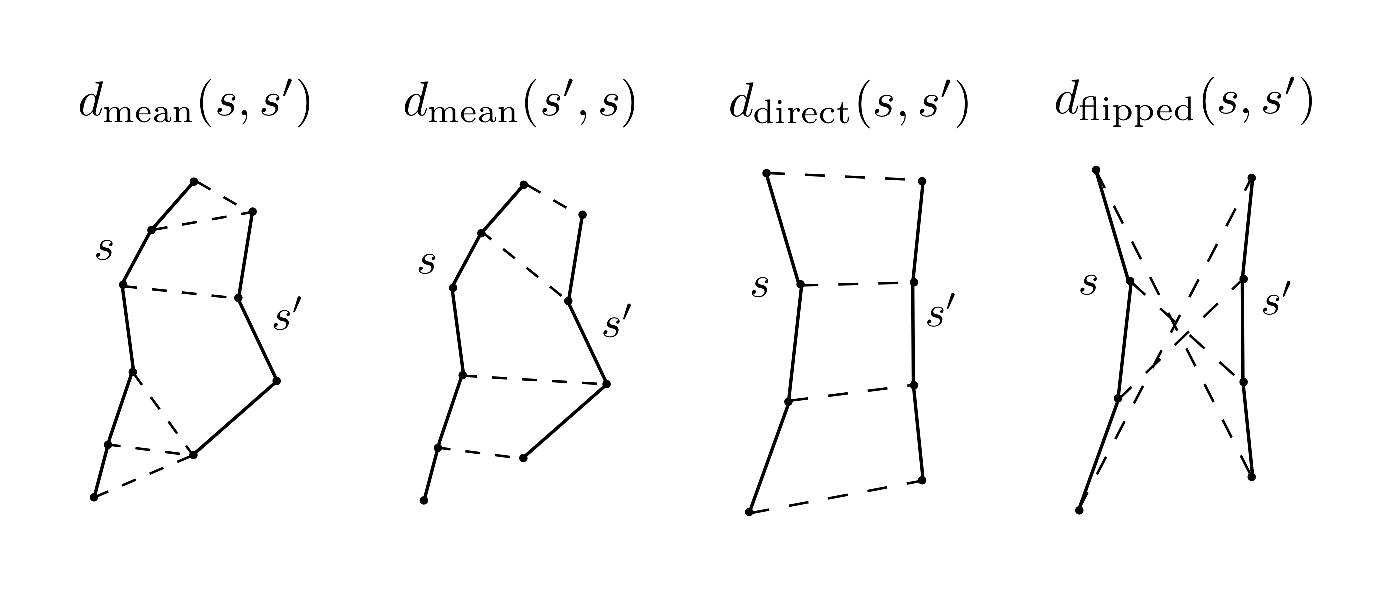
\includegraphics[scale=0.4]{Figures/Fig_2_distances2}
\centering{}
\caption{The principal distance used in this work is minimum average
  direct flip distance
  $\textrm{MDF}=\min(d_{\textrm{direct}},d_{\textrm{flipped}})$ which is
  a symmetric distance function that can deal with the streamline
  bi-directionality problem; it works on streamlines which have the same
  number of points.  Another distance we use is the mean average
  distance which is again symmetric but does not require the streamlines
  to have the same number of points: $\textrm{MAM}_{\textrm{mean}} =
  (d_{mean}(s, s') + d_{mean}(s',s))/2$ (see Eq.~(\ref{eq:mean_average_distance})). 
  In this figure the components of both distances are shown; the streamlines are
  drawn with solid lines, and then with dashed lines we connect the
  pairs of points of the two streamlines whose distances contribute to
  the overall metric. Note that we cannot calculate the $\textrm{MDF}$
  between the streamlines on the left of the figure because they have
  different numbers of points.
  \label{Flo:Distances_used}}
\end{figure}

For these reasons we have opted to use a rather simpler symmetric
distance function~\citep{EGMB10, Visser2010} which we call the minimum
average direct-flip (MDF) distance, see
Eq.~(\ref{eq:direct_flip_distance}). MDF can be applied only when both
streamlines have the same number of points, see
Fig.~\ref{Flo:Distances_used}. Therefore we assume from now on that an initial
discretization of streamlines has been applied, so that all streamlines
have the same number of points $K$, and all segments of
each streamline have equal length. This is a achieved by a simple linear interpolation.

As it has no preferred orientation, a streamline $s=[s_1, s_2, \ldots, s_K]$ is equivalent to
two ordered polylines: $s = (s_1, s_2, \ldots, s_K)$ in $\mathbb{R}^3$
and its flipped version $s^F = (s_K, s_{K-1}, \ldots, s_1)$.  With this
notation the direct, flipped and MDF distances are defined as follows:
\begin{eqnarray}
  d_{\textrm{direct}}(s, t) = d(s, t) & = & \frac{1}{K}\sum_{i=1}^{K}|s_{i}-t_{i}|,\nonumber\\
  d_{\textrm{flipped}}(s, t) & = & d(s,t^F) = d(s^F,t),\nonumber\\
  \textrm{MDF}(s, t) & = & \min(d_{\textrm{direct}}(s, t), d_{\textrm{flipped}}(s, t))\label{eq:direct_flip_distance}.
\end{eqnarray}
\noindent
Here $|x-y|$ denotes the euclidean distance between two points $x$ and
$y$. The direct distance $d_{\mathrm{direct}}(s, t)$ between two
streamlines $s$, and $t$ is the mean of the euclidean distances between
corresponding points. Clearly the MDF distance between two streamlines
of $K$ points requires the calculation of just $2K$ inter-point
distances.

The MDF distance is in fact a metric on the space of streamlines.
Obviously MDF distances are non-negative, are zero if and only if the
two streamlines are identical, and symmetrical.  The triangle inequality
is established as follows. Let $s$, $t$ and $u$ be three streamlines
and assume, without loss of generality, that $d(s,t)$ and $d(t,u)$ actually
minimise the corresponding MDF distances $\mathrm{MDF}(s,t)$ and
$\mathrm{MDF}(t,u)$. (If not, we replace e.g.~$t$ by $t^F$) Then
$\mathrm{MDF}(s, t) + \mathrm{MDF}(t, u) = d(s, t) + d(t, u) \ge d(s,
u)$ (by the triangle inequality for the euclidean distance) $ \ge
\min(d(s,u), d(s, u^F)) = \mathrm{MDF}(s, u)$.

\begin{figure}
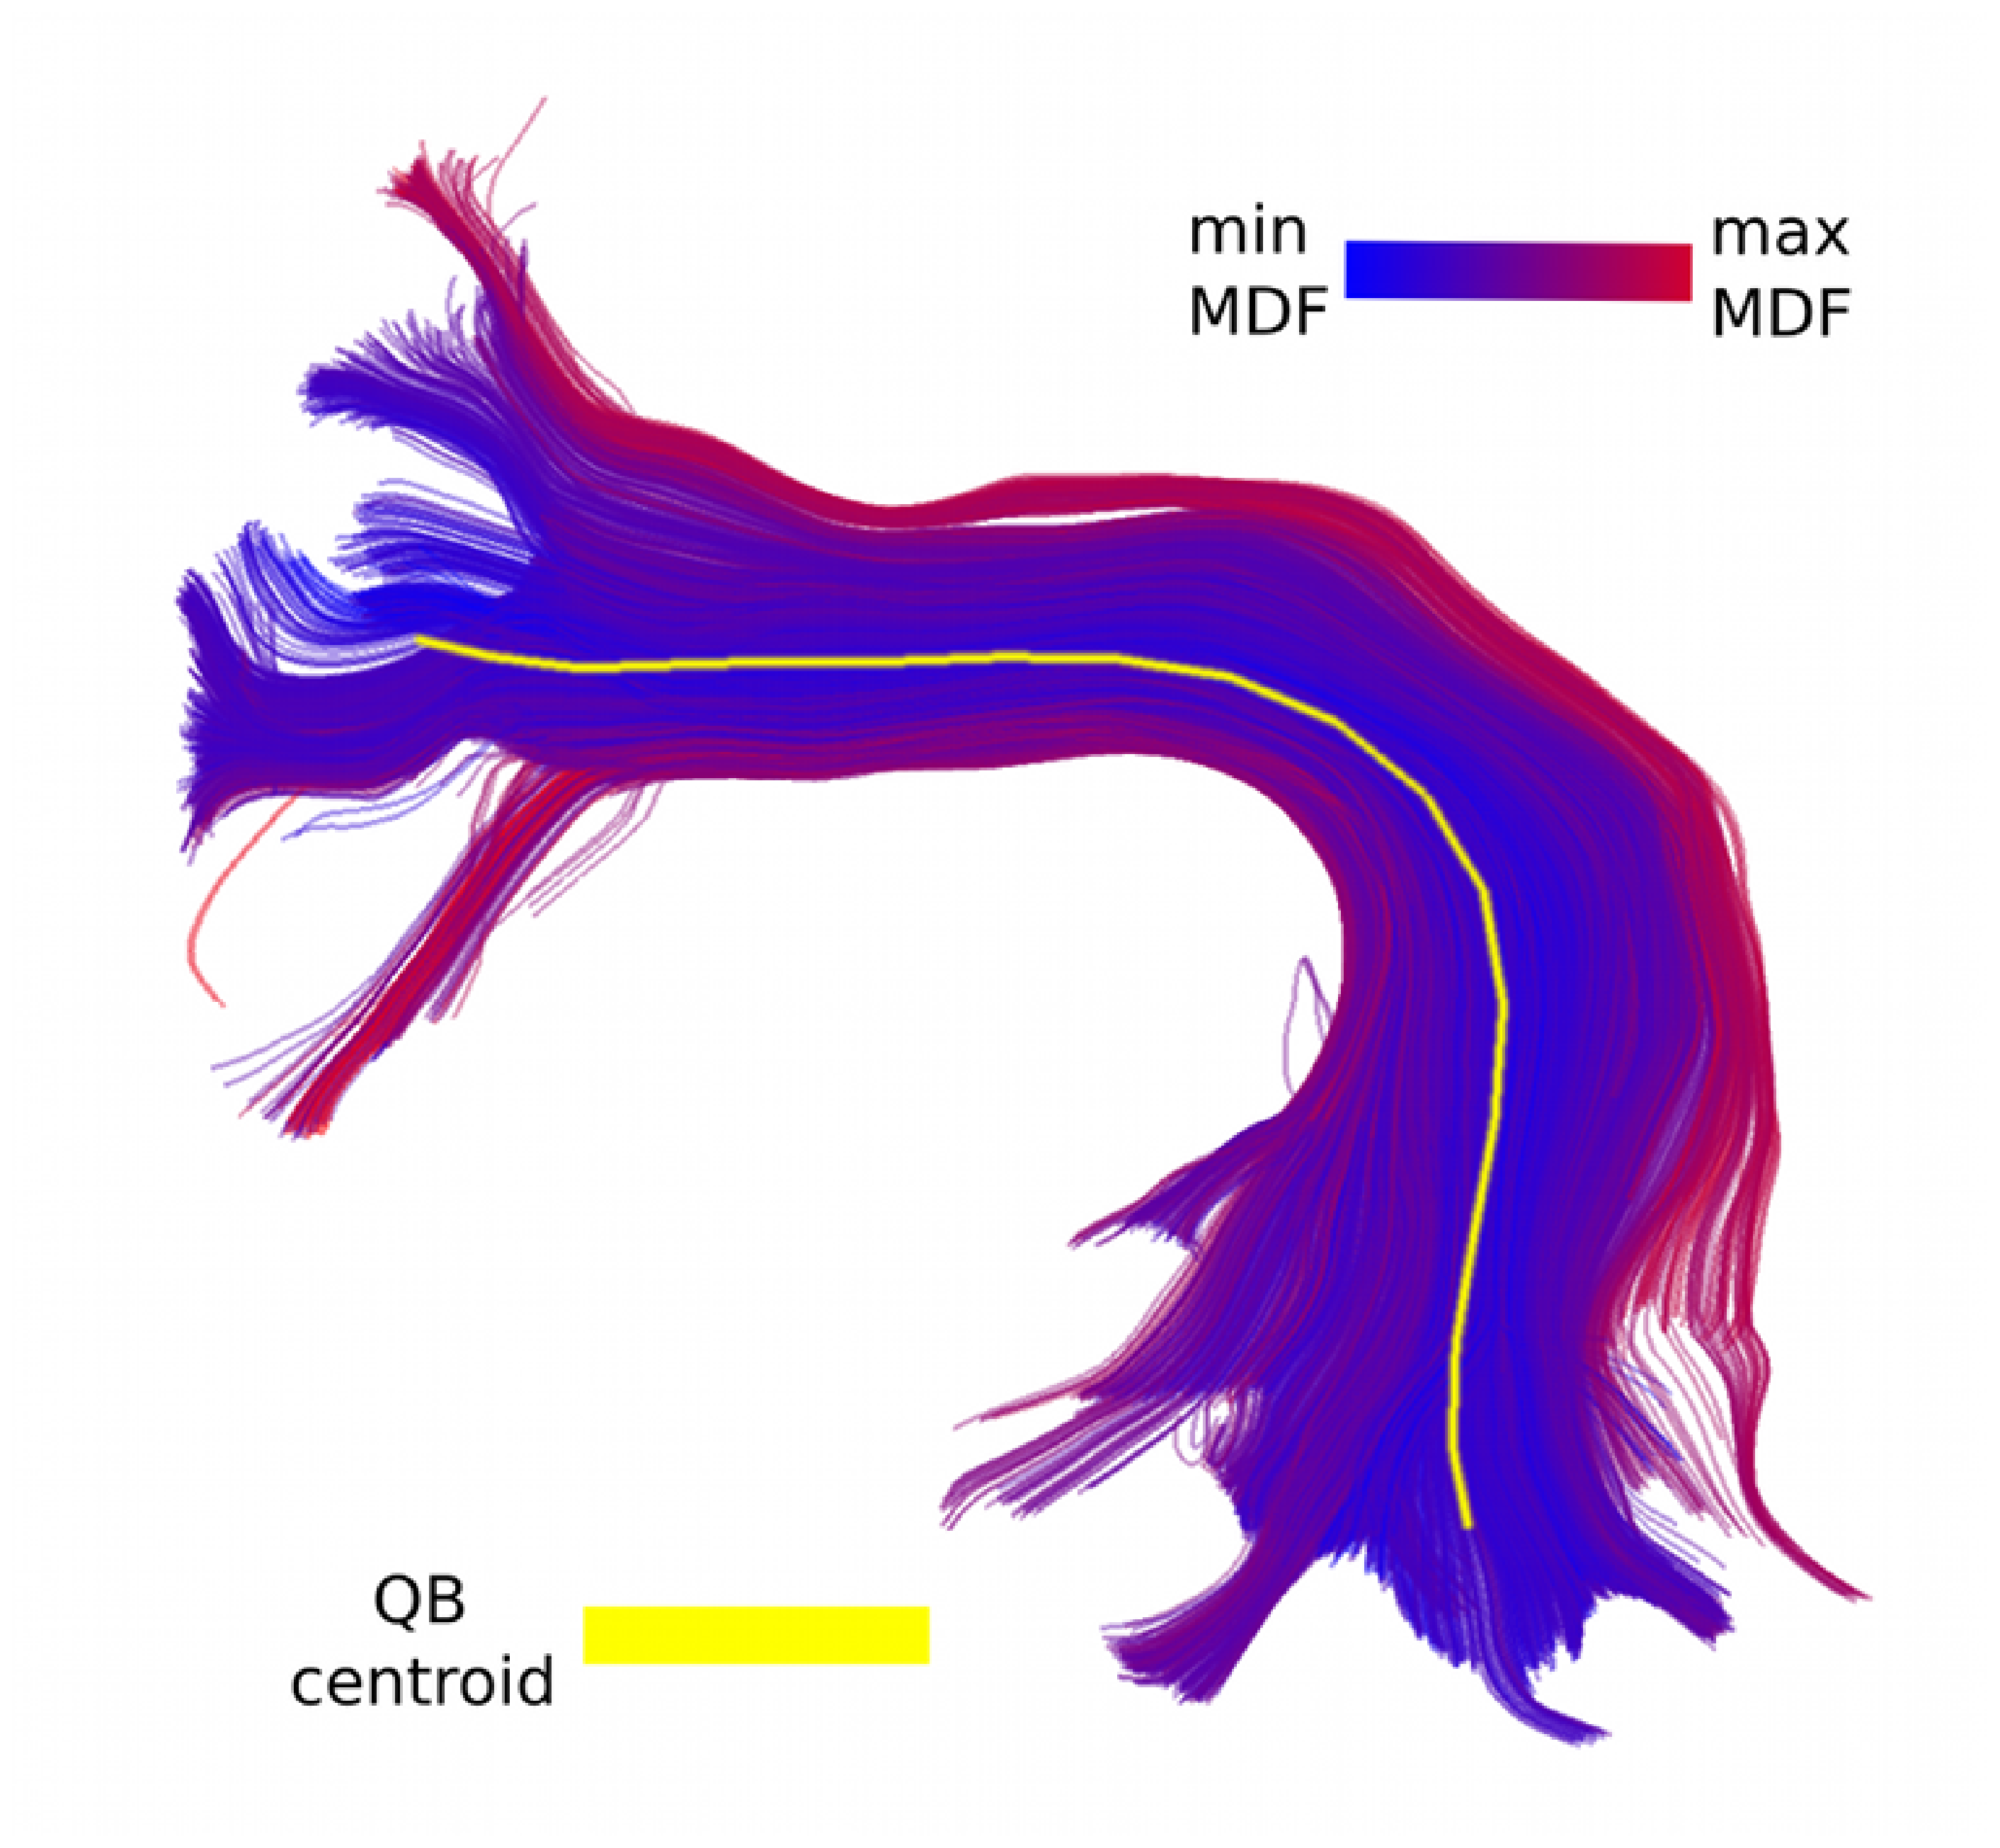
\includegraphics[scale=0.15]{Figures/Fig_11_MDF_arcuate}
\centering{}
\caption{Color coding shows MDF distances from QB centroid to every
  other track in the bundle.\label{Flo:MDF_arcuate}}
\end{figure}


The main advantages of the MDF distance are that it is fast to compute,
it takes account of streamline direction issues through consideration of
both direct and flipped streamlines, and that its behaviour is easy to
understand (see Fig.~\ref{Flo:MDF_arcuate}), from the simplest case of
parallel equi-length streamlines to the most complicated with very
divergent streamline.

Another advantage of the MDF distance function is that it separates
short streamlines from long streamlines; a streamline $s$ that is a
portion of a streamline $s'$ will be relatively poorly matched on MDF to
$s'$. This is consistent with our proposed approach to leave decisions
about the status of short versus long streamlines till after applying a
clustering. At this later stage one can determine whether there are
several similar short streamlines -- perhaps reflecting a damaged fiber
tract -- or localised noise if there are only a few similar streamlines.

A further important advantage of having streamlines with the same number
of points is that we can easily do pairwise calculations on them; for
example add two or more streamlines together to create a new average
streamline. We will see in the next section how streamline addition is a
key property that we exploit in the QB clustering algorithm.

Care needs to be given to choosing the number of points required in a
streamline (streamline discretization). We always keep the endpoints
intact and then discretize into segments of equal lengths. One
consequence of short streamlines having the same number of points as
long streamlines is that more of the curvature information from the long
streamlines is lost relative to the short streamlines i.e. the short
streamlines will have higher resolution.  We found empirically that this
is not an important issue and that for clustering purposes even
discretizing to only $K=3$ points per streamline can produce useful clusterings \citep{EGMB10}. Depending on the application, more or fewer points can
be used. In the results presented we often use $K=12$ which achieves a
good trade-off between streamline resolution and memory size
reduction.

In some later stages in the analysis of tractographies. e.g.~for merging
clusters, we find a use for Hausdorff-type distance functions which for
simplicity we denote as MAM distances -- short for Minimum (or Maximum,
or Mean) Average Minimum distance (MAM). (In this nomenclature the
classical Hausdorff distance is the Maximum Average Minimum distance.)
We mostly use the Mean version of this family, see
Eq.~(\ref{eq:mean_average_distance}) but the others are potentially
useful as they can weight different properties of the streamlines. As
noted above, these distances are slower to compute but they can work
with different number of segments on streamlines; this is useful for
some applications. The equations below show the formulation of these
distances:
\begin{eqnarray}
d_{\textrm{mean}}(s,s') & = & \frac{1}{K_{A}}\sum_{i=1}^{K}d(x_{i},s'),\nonumber \\
d_{\textrm{min}}(s,s') & = & \min_{i=1,...,K}d(x_{i},s'),\qquad\textrm{and}\label{eq:minimum_distance}\\
d_{\textrm{max}}(s,s') & = & \max_{i=1,...,K }d(x_{i},s'),\qquad\textrm{where}\label{eq:maximum distance}\\
d(x,s') & = & \min_{j=1,...,K'}|x-x_{j}'|.\nonumber \\
\textrm{MAM}_{\textrm{min}} & = & \min(d_{\textrm{mean}}(s,s'),d_{\textrm{mean}}(s',s))\label{eq:min_average_distance}\\
\textrm{MAM}_{\textrm{max}} & = & \max(d_{\textrm{mean}}(s,s'),d_{\textrm{mean}}(s',s))\nonumber \\
\textrm{MAM}_{\textrm{mean}} & = & (d_{\textrm{mean}}(s,s')+d_{\textrm{mean}}(s',s))/2\label{eq:mean_average_distance}\end{eqnarray}


\noindent
where the number of points $K$ and $K'$ on the two streamlines are not
necessarily the same. For the same distance value $\textrm{MAM}_{\textrm{min}}$, $\textrm{MAM}_{\textrm{max}}$ and $\textrm{MAM}_{\textrm{mean}}$ will give different results. For example,
$\textrm{MAM}_{\textrm{min}}$ will bring together more short streamlines
with long streamlines than $\textrm{MAM}_{\textrm{max}}$, and
$\textrm{MAM}_{\textrm{mean}}$ will have an in-between effect.  Other
distances than $d(x_{i},s')$ can be used in
Eq.~\ref{eq:minimum_distance} and Eq.~\ref{eq:maximum distance}.
However, we have not investigated them in this work in relation to
clustering algorithms.

\subsection{The QB algorithm\label{sub:QB-description}}

QuickBundles (QB) is a surprisingly simple and very fast algorithm which
can reduce tractography representation to an accessible structure in a
time that is linear in the number of streamlines $N$. QB is an extended
update on our preliminary work~\citet{EGMB10}. By the term
\emph{bundle} we mean here streamlines which are in close proximity
according to a streamline-based distance, therefore, they have similar
spatial and shape characteristics and not necessarily direct
correspondence to neuroanatomical bundles (tracts).

In QB each item, a streamline, is a fixed-length ordered sequence of
points in $\mathbb{R}^{3}$, and QB uses comparison functions and
amalgamations which take account of and preserve this structure.
Moreover each item is either added to an existing cluster on the basis
of the distances between the cluster descriptor of the item and the
descriptors of the current list of clusters. Clusters are held in a list
which is extended according to need. Unlike amalgamation clustering
algorithms such as $k$-means~\citep{steinhaus1956division,
  macqueen1967some} or BIRCH~\citep{zhang1997birch}, there is no
reassignment or updating phase in QB -- once an item is assigned to a
cluster it stays there, and clusters are not amalgamated. QB derives its
speed and efficiency from this idea.

A clustering algorithm needs a measure of distance between two
streamlines, and QB uses a particular distance measure that we call
minimum average direct flip (MDF).  The MDF measure requires that each
streamline be resampled to have $K$ points. We have described the MDF measure
and the resampling in section~\ref{sub:track-distances}.

QB stores information about clusters in \emph{cluster nodes}. We index
the streamlines with $i = 1 \dots N$ where $s_{i}$ is the $K\times3$
matrix representing streamline $i$.  A cluster node is defined as a
triple $c=(I,h,n)$ where $I$ is the list of the integer indices $i = 1
\dots N$ of the streamlines in that cluster, $n$ is the number of
streamlines in the cluster, and $h$ is the \emph{streamline sum}. $h$ is
a $K \times3$ matrix which can be updated online when a streamline is
added to a cluster and is equal to:
\begin{equation}
  h=\sum_{i=1}^{n}s_{i}
\end{equation} 
where $s_{i}$ is the $K\times3$ matrix representing streamline $i$,
$\Sigma$ here represents matrix addition, and $n$ is the number of
streamlines in the cluster. One summary of the cluster node is the
centroid streamline $v$ where:
\begin{equation}
  v = h / n
\end{equation}
An example of the QB centroid is presented in Fig.~\ref{Flo:MDF_arcuate}.
%\begin{float}
\begin{algorithm}[h]
%\begin{boxedalgorithmic}
\begin{algorithmic}
\REQUIRE $T=\{s_{1},...,s_{i},...,s_{N}\}$, $\theta$
\ENSURE $C=[c_{1},...,c_{k},...,c_{M}]$ 
\STATE \# create first cluster
\STATE $c_{1} \leftarrow ([1],s_{1},1)$
\STATE $C\leftarrow[c_{1}]$
\STATE $M\leftarrow1$ 
\FOR{$i=2$ to $N$}
	\STATE $t\leftarrow s_{i}$
	\STATE $\texttt{alld}\leftarrow\textbf{infinity}(M)$ \# distance buffer
	\STATE $\texttt{flip}\leftarrow\textbf{zeros}(M)$ \# flipping check buffer
	\FOR{$k=1$ to $M$ }
		\STATE $v\leftarrow c_{k}.h/c_{k}.n$
		\STATE $d\leftarrow d_{\textrm{direct}}(t,v)$
		\STATE $f\leftarrow d_{\textrm{flipped}}(t,v)$
	\STATE \# evaluate MDF
	\IF{$f$ < $d$}
		\STATE $d \leftarrow f$
		\STATE $\texttt{flip}_{k} \leftarrow 1$
	\ENDIF
	\STATE $\texttt{alld}_{k} \leftarrow d$
	\ENDFOR
\STATE $m\leftarrow \min(\texttt{alld})$
\STATE $l\leftarrow \mathrm{arg min}(\texttt{alld})$
\IF{$m < \theta$} 
\STATE \# append to current cluster
	\IF{$\texttt{flip}_{l}$ is $1$} 
		\STATE $c_{l}.h \leftarrow c_{l}.h + t^F)$
	\ELSE
		\STATE $c_{l}.h \leftarrow c_{l}.h + t$
	\ENDIF
	\STATE $c_{l}.n \leftarrow c_{l}.n + 1$
	\STATE \textbf{append}($c_{l}.I$,$i$)
\ELSE 
\STATE \# create new cluster
        \STATE $c_{M+1} \leftarrow ([i],t,1)$
        \STATE \textbf{append}$(C,c_{M+1})$
	\STATE $M\leftarrow M+1$
\ENDIF
\ENDFOR 
\end{algorithmic}
%\end{boxedalgorithmic}
\caption{QuickBundles}
\label{Alg:QuickBundles}
\end{algorithm}

The algorithm proceeds as follows.  At any one step in the algorithm we
have $M$ clusters. Select the first streamline $s_{1}$ and place it in
the first cluster $c_{1}\leftarrow(\{1\}, s_{1},1)$; $M=1$ at this
point.  For each remaining streamline in turn $i = 2 \dots N$: (i)
calculate the MDF distance between streamline $s_{i}$ and the centroid
streamlines $v_{e}$ of all the current clusters $c_{e}$, $e = 1 \dots
M$, where $v$ is defined on the fly as $v=h/n$; (iii) if any of the MDF
values $m_{e}$ are smaller than a distance threshold $\theta$, add
streamline $i$ to the cluster $e$ with the minimum value for $m_{e}$;
$c_{e}=(I,h,n)$, and update $c_{e}\leftarrow(\mathbf{append}(I,i), h+s,
n+1)$; otherwise create a new cluster $c_{M+1}\leftarrow([i],s_{i},1)$,
$M\leftarrow M+1$.

Choice of orientation can become an issue when adding streamlines
together, because streamlines can equivalently have their points ordered
$1 \dots K$ or be flipped with order $K \dots 1$.  A step in QB takes
account of the possibility of needing to perform such a flip of a
streamline before adding it to a centroid streamline according to which
direction produced the MDF value.

The complete QB algorithm is described in formal detail in
Algorithm~\ref{Alg:QuickBundles}.  One of the reasons why
QB has on average linear time complexity derives from the structure of
the cluster node: we only save the sum of current streamlines
$h$ in the cluster and the sum is cumulative; moreover there is
no recalculation of clusters, the streamlines are passed through only
once and a streamline is assigned to one cluster only.

\subsection{The QB Representation\label{QB_Representation}}

One of the major benefits of applying QB to tractographies is that it
can provide meaningful simplifications and find features that were
previously invisible or difficult to locate because of the high density
of the tractography. For example we used QB to cluster part of the
corticospinal tract (CST). This bundle was labelled in the datasets
provided by PBC (\ref{sub:QB-Data-sets}) and it was selected by an
expert. The QB representation is clearly shown in Fig.~\ref{Flo:cst_pbc}
where every cluster is represented by a single centroid streamline. To
generate this clustering we used a tight threshold of $10$~mm. We
observe that only a few centroid streamlines travel the full distance
from bottom to top and that they are many streamlines that are broken
(i.e. shorter than what was initially expected) or highly divergent.

Another interesting feature of QB is that it can be used to merge or
split different structures by changing the distance threshold.  This is
shown in Fig.~\ref{Flo:simulated_orbits}; on the left we see simulated
paths made from simple sinusoidal and helicoidal functions packed
together. The colour coding is used to distinguish the three different
structures. With a lower threshold the three different structures remain
separated but when we use a higher threshold the red and blue bundles
are represented by only one cluster indicated by the purple centroid
streamline.

\begin{figure*}
\begin{centering}
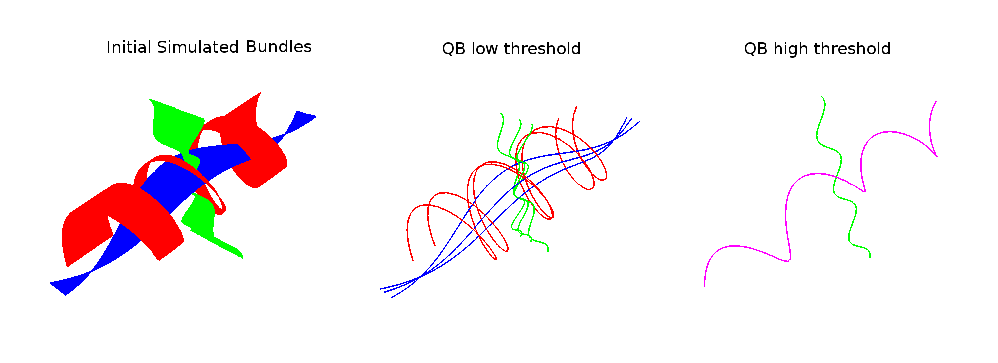
\includegraphics[width=160mm]{Figures/Fig_5_helix_phantom}
\par\end{centering}
\caption{Left: $3$ bundles of simulated trajectories; red, blue and
  green consisting of $150$ streamlines each. All $450$ streamlines are
  clustered together using QB. Middle and Right: centroid streamlines
  using thresholds $1$ and $8$ respectively.  At low threshold the
  underlying structure is reflected in a more detailed
  representation. At higher threshold, closer bundles merge
  together. Here the red and blue bundle have merged together in one
  cluster represented by the purple centroid
  streamline.\label{Flo:simulated_orbits}}
\end{figure*}

We can see similar effects with real streamlines, for instance those of
the fornix shown at the left panel of Fig.~\ref{Flo:QB_fornix} where we
can obtain different numbers of clusters at different thresholds. In
that way we can stress thinner or thicker sub-bundles contained inside
other bigger bundles.

\begin{figure*}[htp]
\centerline{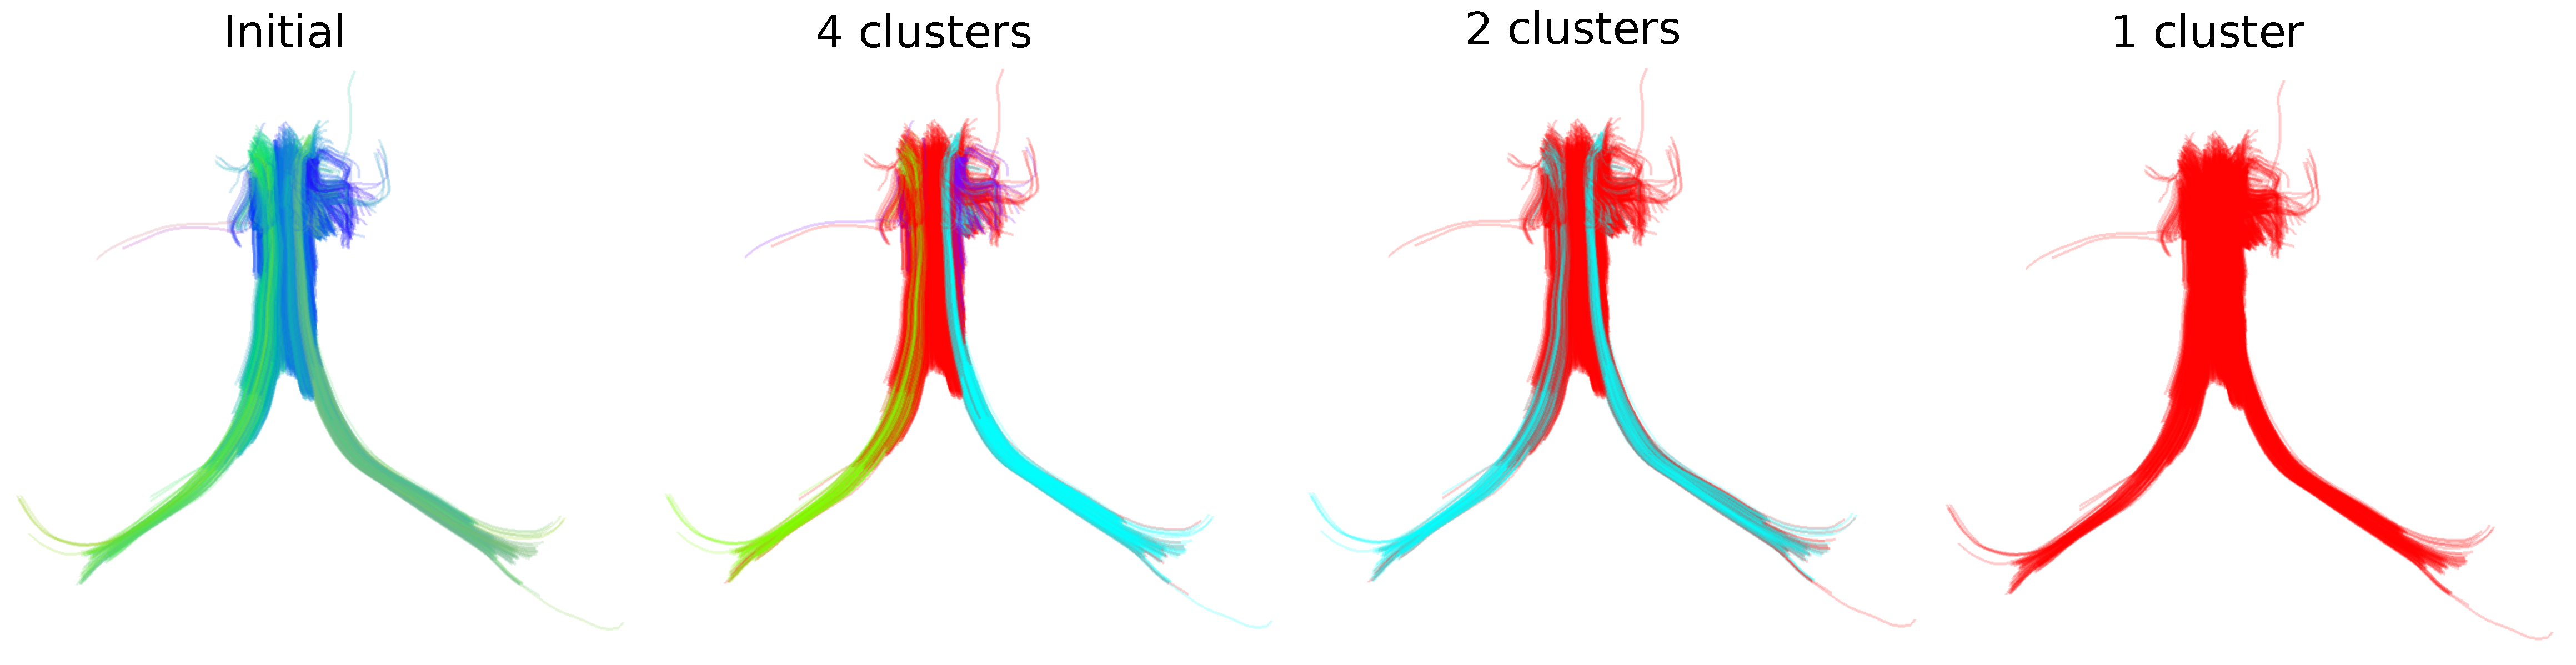
\includegraphics[width=160mm]{Figures/Fig_6_QB_fornix}}
\caption{QB clustering of the Fornix bundle. The original Fornix
  ($1076$ streamlines) is shown on the left panel using a standard
  orientation colormap. We observe that the Fornix consists of two long
  distant legs (left and right Fimbria) and a thicker upper part (Body
  of Fornix). We show here how QB will be able to distinguish the parts
  of the Fornix at different resolutions. With a $15$~mm threshold QB
  generates 4 clusters shown on the second panel with distinct
  colors. Here the left and right Fimbria are clearly distinguished from
  the Body. A last cluster (with blue) exposes a shorter part of the
  Body which is probably due to noise in the data. With a $18$~mm
  threshold only two clusters are created. Both Fibria are brought
  together as one cluster. A property useful for studies which want to
  use both Fimbria as one. With a $20$~mm threshold the entire Fornix is
  one cluster. This is useful for interactive applications because now
  the entire Fornix can be described by only one centroid streamline. The streamlines of the Fornix were discretized to have $18$
  points.\label{Flo:QB_fornix}}
\end{figure*}

In order to quantify the dimensionality reduction it achieves we applied
QB clustering to the 10 human subject datasets (\ref{sub:QB-Data-sets}). The mean
data compression (ratio of tractography size to number of QB clusters)
was $34.4:1$ with a $10$~mm threshold and $230.4:1$ with a $20$~mm
threshold.

\subsection{Comparison of clusterings\label{sub:Tightness-comparisons-1}}

We have found rather few systematic ways available in the literature to
directly compare different clustering results for tractographies, beyond
that of \citet{moberts2005evaluation} who quantified the agreement
between a clustering and a `gold standard' tractography labelled by
their team.  We have used a more symmetrical measure of agreement
between two clusterings that do not require a prior labelled dataset.
It is called the \emph{optimised matched agreement} (OMA). As with the
\emph{adjusted Rand index} (ARI)~\citep{moberts2005evaluation}, OMA requires
the calculation of the $M \times N$ streamline cross-classification
matrix $X=(x_{ij})$. The entries of $X$ are the counts of the number of streamlines in all
pairwise intersections of clusters, one from each of the two
clusterings.  If $\mathcal{A}=\{A_i:i=1\dots M\}$ and
$\mathcal{B}=\{B_j:j=1\ldots N\}$ are the two clusterings, then
$x_{ij}=|A_i \cap B_j|$. As there is no \emph{a priori} correspondence
or \emph{matching} between the clusters in $\mathcal{A}$ and those in
$\mathcal{B}$, and vice versa, we need to find one empirically. If
$j=\pi(i)$ is a possible matching then the corresponding \emph{matched
  agreement} is $\mathrm{MA}(\pi) = \sum_{i=1}^M x_{i,\pi(i)}$. A
matching $\pi$ that yields OMA by maximising $\mathrm{MA}(\pi)$ can be
found using the Hungarian Algorithm~\citep{Kuhn1955}. The interpretation
of the OMA statistic is analogous to that of the well-known Kappa
measure of inter-rater agreement~\citep{altman1995}, with the range 61\%
to 80\% corresponding to a `good' strength of agreement.

We will use OMA to compare the different clusterings that arise when the
streamlines in the tractography are shuffled. However this statistic has
its limitations. Not only are there considerable computational overheads
in calculating the cross-classification matrix, there is also a
fundamental disadvantage because they do not work with clusterings of
different tractographies. Being able to compare results of clusterings
across brains is crucial for creating stable brain imaging procedures,
and therefore it is necessary to develop a way to compare different
tractography clusterings on different sets of streamlines from the same
or different subjects.

Although we recognise that these are difficult problems, we propose the
following approach with three novel comparison functions which we call
\emph{coverage}, \emph{overlap} and \emph{bundle adjacency}. These
metrics aim to quantify how well a data reduction performs. Ideally most
points of the full dataset should be near to the reduced set
(coverage), but not too many (overlap).

Let $S$ and $T$ be two sets of streamlines, and let $\theta>0$ be a
selected threshold. We will say that $s \in S$ is
$\theta$-\emph{approximated} by $T$ if there is at least one streamline
$t \in T$ with $\mathrm{MDF}(s,t)\le \theta$. We define coverage of $S$
by $T$ as the fraction of $S$ that is $\theta$-approximated by $T$. Coverage
ranges between 0 (when all streamlines in $S$ are too far from $T$) and
1 (when every streamline in $S$ is $\theta$-approximated by $T$).

We define the \emph{overlap} of $T$ in $S$ as the average number of
approximating streamlines in $T$ that for $\theta$-approximate
streamlines in $S$.  Overlap is undefined of no streamlines in $S$ are
approximated by $T$, otherwise it can take any value greater then or
equal to 1, with higher values indicating the degree of redundancy of
$T$ in $S$; if $T$ has several similar streamlines then this will tend
to boost overlap.

Coverage and overlap measure how well one set approximates another. In
order to compare two reductions of possibly different datasets we
define the symmetric measure \emph{bundle adjacency} (BA).  BA is the
average of the coverage of $T$ by $S$ and the coverage of $S$ by
$T$: $$\mathrm{BA}(S,T) = (\mathrm{coverage}(S,T) +
\mathrm{coverage}(T,S))/2.$$ BA ranges between 0, when no streamlines of
S or T have neighbours in the other set, and 1 when they all do.

\subsection{\label{sub:QB-Data-sets}Data sets}

We applied QuickBundles to a variety of datasets: simulations, $10$
human tractographies collected and processed by ourselves, and one
tractography with segmented bundles which was available online.

\textbf{Simulated trajectories.} We generated $3$ different bundles of
parametric paths sampled at $200$ points. The streamlines were made from
different combinations of sinusoidal and helicoidal functions.  Each
bundle contained 150 streamlines.  For the red bundle in
Fig.~\ref{Flo:simulated_orbits} a pencil of helical streamlines all
starting at the same point on a cylinder was generated by linearly
varying the pitch of the helices; the green bundle was made up from a
divergent pencil of rays on a sinusoidally corrugated sheet; the blue
bundle is similarly made from a divergent rays on a sinsusoidally
corrugated sheet, with the rays undergoing sinusoidal modulated lateral
bending over a range of amplitudes.

\textbf{Human subjects.} We collected data from $10$ healthy subjects at
the Medical Research Council's Cognition and Brain Sciences Unit with a 3~Tesla
scanner (TIM Trio, Siemens), using a Siemens advanced diffusion
work-in-progress sequence, and STEAM \citep{merboldt1992diffusion,MAB04}
as the diffusion preparation method. The field of view was
$240\times240\,\textrm{mm}^{2}$, matrix size $96\times96$, and slice
thickness $2.5\,\textrm{mm}$ (no gap).  $55$ slices were acquired to
achieve full brain coverage, and the voxel resolution was
$2.5\times2.5\times2.5\,\textrm{mm}^{3}$. A $102$-point half grid
acquisition \citep{Yeh2010} with a maximum $b$-value of $4000\,
\textrm{s/mm}^{2}$ was used.  The total acquisition time was $14'\,21''$
with TR=$8200\,\textrm{ms}$ and TE=$69\,\textrm{ms}$. The experiment was
approved by the Cambridge Psychology Research Ethics Committee (CPREC).

For the reconstruction of the $10$ human datasets we used Generalized
Q-Sampling \citep{Yeh2010} with diffusion sampling length $1.2$ and for
the tractography propagation we used EuDX (Euler integration with
trilinear interpolation, \citet{Garyfallidis_thesis}), angular threshold
\ang{60}, total weighting $0.5$, propagation step size $0.5$ and
quantitative anisotropy stopping threshold $0.0239$ (see
Fig.~\ref{Flo:arcuate_close}).

\textbf{PBC human subjects}. We also used labelled datasets by
experts(see Fig.~\ref{Flo:cst_pbc} and \ref{Flo:QB_fornix}), from the
freely available tractography database used in the Pittsburgh Brain
Competition Fall $2009$, ICDM (pbc.lrdc.pitt.edu).

\end{methods}

\section{Results}

In this section we justify our claims about the speed and linear
complexity of QB (\ref{sub:Complexity}). Next we demonstrate the
robustness of QB as a method for clustering tractographies
(\ref{sub:Comparisons}). In \ref{sub:group_comp} we show a new way to
find similarities across different tractographies and
in \ref{sub:short_tracks} we discuss about some potential limitations
of our methods and possible workarounds.

\subsection{Complexity and timings\label{sub:Complexity}}

The execution time of QB is affected by the following parameters: $K$,
the fixed number of discretized points per streamline; $\theta$ the
distance threshold, which controls the heterogeneity of clusters; and
$N$ the size of the subset of the tractography on which the clustering
will be performed. When $\theta$ is higher, fewer more heterogeneous
clusters are assembled, and conversely when $\theta$ is low, more
clusters of greater homogeneity are created.

The complexity of QB is in the best case linear time $\mathcal{O}(N)$
with the number of streamlines $N$ and worst case $\mathcal{O}(N^{2})$
when every cluster contains only one streamline. The average case is
$\mathcal{O}(MN)$ where $M$ is the number of clusters however because
$M$ is usually much smaller than $N$ ($M\ll N$) we can neglect $M$ and
denote it only as $\mathcal{O}(N)$ as it is common in complexity
theory. We created the following experiment to investigate this claim
and we found empirically that the average case is actually
$\mathcal{O}(N)$ for tractographies (see Fig.\ref{Flo:Speed1}).  In this
experiment we timed the duration of QB clustering of tractographies
containing from \num{50000} to \num{500000} streamlines in steps of
\num{50000}, with $12$ points per streamline and different QB thresholds
($20,25,30$~mm). These results were obtained using a single thread
Intel(R) CPU E5420 at 2.50GHz on a standard notebook. The results for a
single subject can be seen in Fig.~\ref{Flo:Speed1}. The same pattern
was observed for the remaining $9$ subjects. This experiment concludes
that QB is suitable for fast and linear time clustering of
tractographies.

\begin{figure}
\noindent \begin{centering}
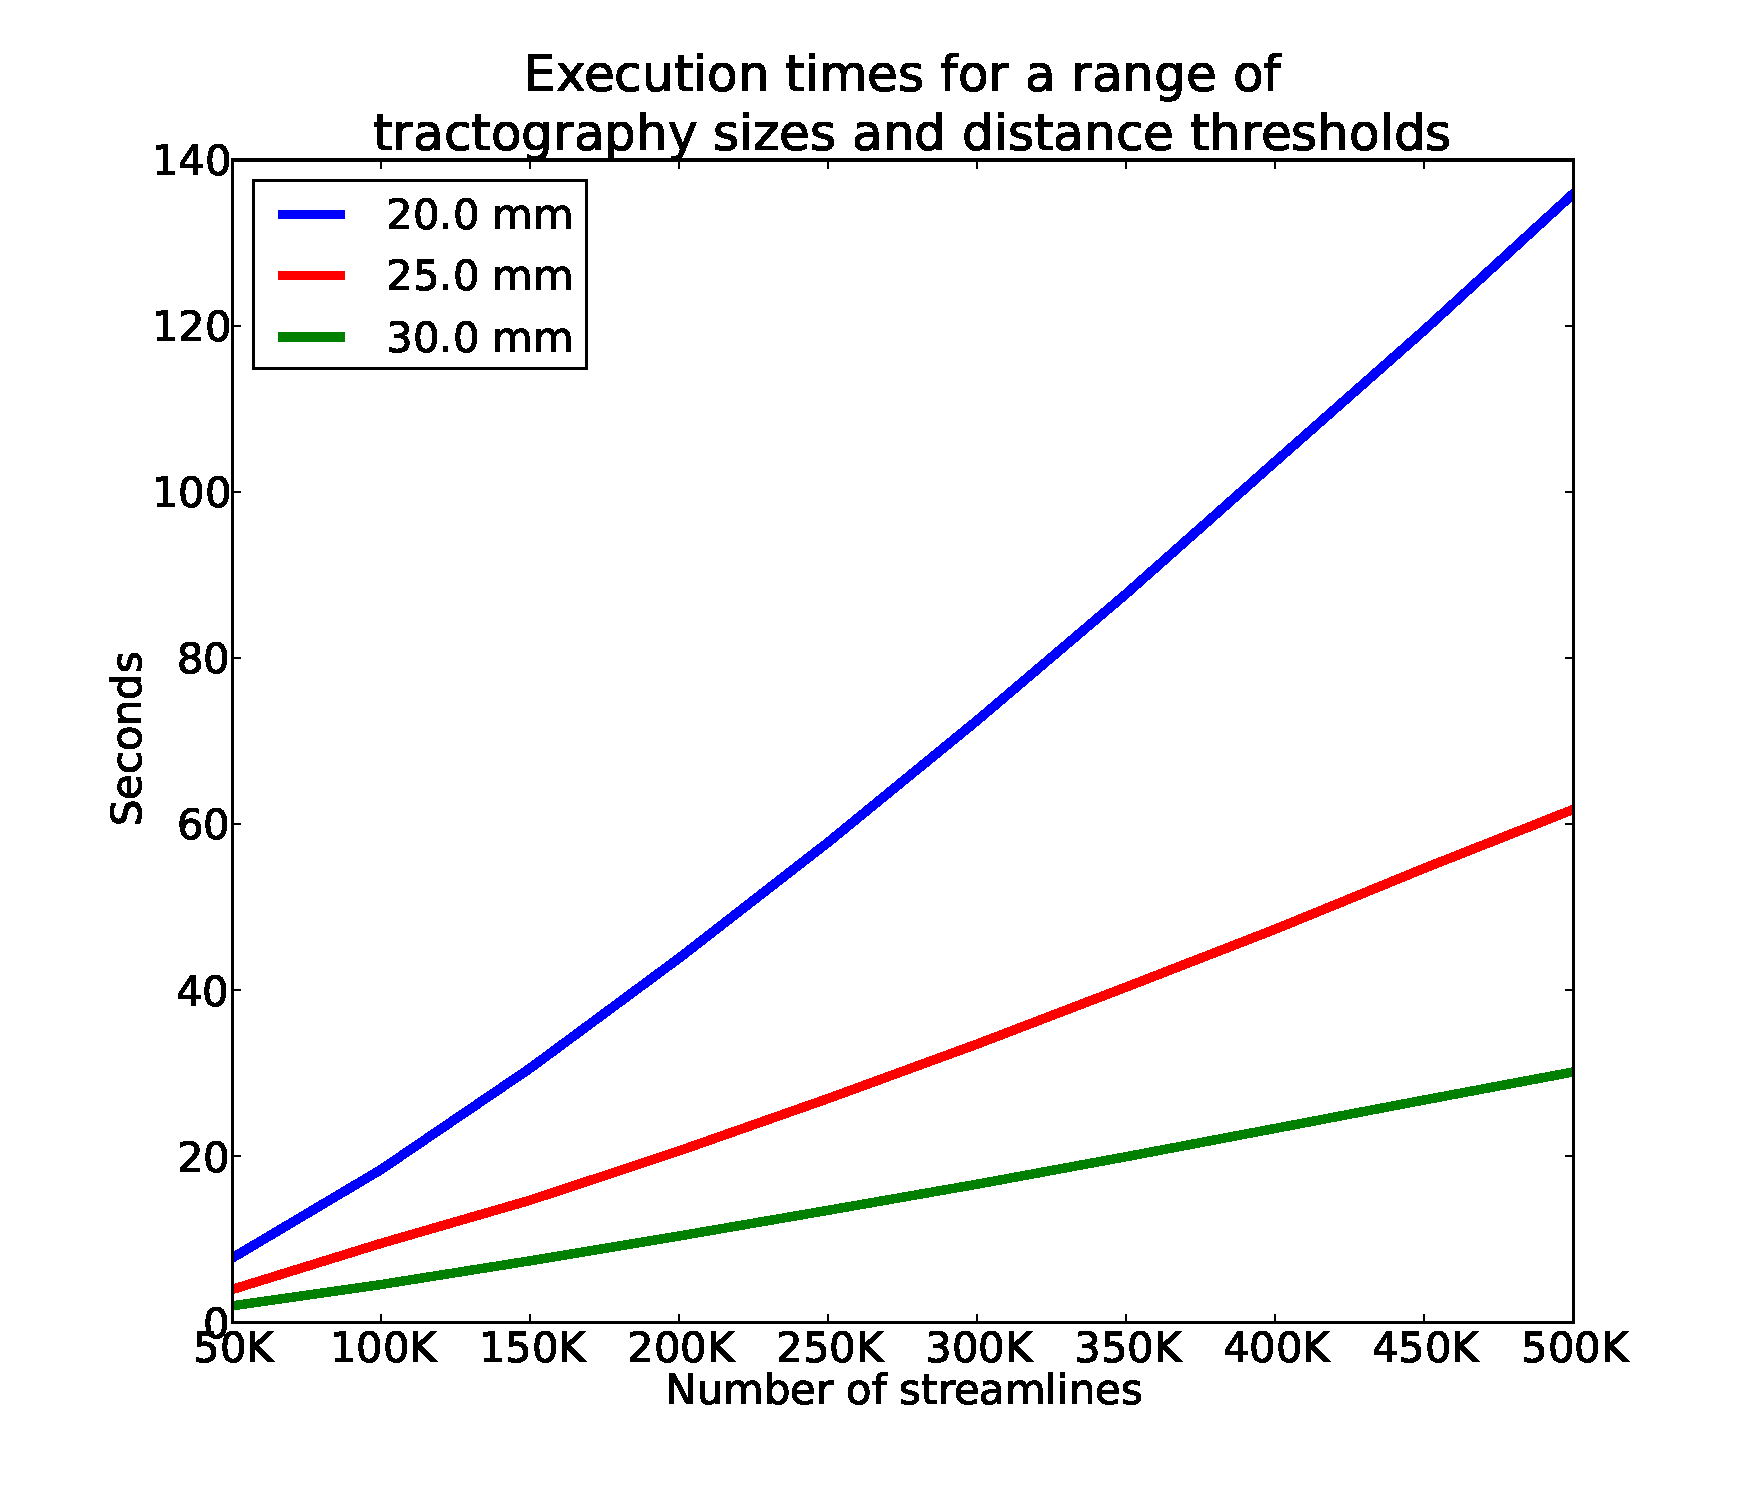
\includegraphics[scale=0.3]{Figures/Fig_3_timings}
\par\end{centering}
\caption{Time comparisons of QB using different distance thresholds and
  different number of streamlines. Time increases linearly as the number
  of streamlines increases. \label{Flo:Speed1}}
\end{figure}

As a further test we compared QB (with $12$ point streamlines and a
distance threshold of $10$~mm) with timings reported from the fastest
state of the art methods found in the literature. These methods have different goals that those of QB however we think that it is useful to show the important speedup that QB offers for the same number of streamlines. With $\num{1000}$
streamlines \citet{wang2010tractography}'s algorithm took $30$s whereas
QB took $0.07$s.  $\num{14400}$ seconds were required for the same method of to cluster $\num{60000}$ streamlines; QB
took $14.7$s.  In a third study a substantial tractography of size $\num{400000}$ was clustered by \citet{Visser2010} in
$\num{75000}$s; QB completed this task in only $160.1$s. The speed-up factors in these three comparisons were $429$, $980$ and $468$ respectively. Therefore, we  see the valuable speedup that QB achieves, holding out the prospect of real-time (less than 1~second) clustering on datasets of up to \num{20000} streamlines.

\subsection{Stability of QB \label{sub:Comparisons}}

One of the disadvantages of most clustering algorithms is that they give
different results with different initial conditions; for example this is
recognised with k-means, expectation-maximization
\citep{dempster1977maximum} and k-centers \citep{gonzalez1985clustering}
where it is common practice to try a number of different random initial
configurations. The same holds for QB so if there are not distinct
clusters such that the distance between any pair of clusters is
supra-threshold and the diameter of all clusters is sub-threshold, then
with different permutations of the same tractography we will typically
see similar number of clusters but different underlying clusters. We
will examine the robustness of QB in this respect.

As a first step we recorded the numbers of QB clusters in $20$ different
random permutations of the tractographies of $10$ human subjects acquired
as described in section \ref{sub:QB-Data-sets}. We first removed short
streamlines shorter than $40$~mm and discreatized the streamlines at $12$
points. Then we applied QB with threshold at $10$~mm. The mean number of
clusters was $2645.9$ (min $1937.6$; max $3857.8$; s.d.~$653.8$). There
is therefore a considerable between-subject variation in this metric. By
contrast the within-subject variability of the number of clusters across
random permutations is rather small, with mean standard deviation $12.7$
(min $7.3$; max $17.4$). This suggests a good level of consistency in
the data reduction achieved by QB.

Next we investigated how consistent QB clusterings are when datasets
are re-ordered. Twelve different random permutations were generated for each
of $10$ tractographies and the corresping QB clusterings were computed
with MDF threshold $10$~mm. For each subject the $66$ pairings of QB
clusterings were compared using the optimised matched agreements index
and then averaged. Across subjects the mean OMA
(\ref{sub:Tightness-comparisons-1}) was 74.1\% ($\pm 0.39$\%) which can
be interpreted as a good level of agreement~\citep{altman1995}.

As well as checking that QB created sets of centroids with good coverage
and overlap statistics, we went on to show that the performance of QB
generalises to sets of streamlines different from the training set, and
is superior to a random sample of streamlines. We split each of the 10
tractographies randomly into two halves $T_1$ (training set) and $T_2$
(test set). The QB clustering at distance threshold $10$~mm was derived
for $T_1$. Denote by $C_1$ and $c_1$ the set of centroids and the number
of them. Let $R_1$ be a random subset of $T_1$ of size $c_1$. Using the
measures described in section~\ref{sub:Tightness-comparisons-1} we found
that with distance threshold $10$~mm the mean coverage (s.d.) of $T_1$
by $C_1$ was $99.96$\% ($\pm 0.007$\%), of $T_2$ by $C_1$ was $99.31$\%
($\pm 0.08$\%) and of $T_2$ by $R_1$ was $90.49$\% ($\pm 0.41$\%). The mean
overlap (s.d.) at this threshold of $C_1$ in $T_1$ was $2.44$ ($\pm
0.08$), of $C_1$ in $T_2$ was $2.44$ ($\pm 0.08$), and of $R_1$ in $T_2$
was $5.57$ ($\pm 0.50$).

The same analysis was performed with QB clusterings with distance
threshold $20$mm and comparing against streamlines which had again $20$mm MDF
distance from the representatives. (Note that though
we have selected the same values here for the two thresholds they do not
have to be the same.) We found that with distance threshold $10$mm the
mean coverage (s.d.) of $T_1$ by $C_1$ was $99.99$\% ($\pm 0.004$\%), of
$T_2$ by $C_1$ was $99.91$\% ($\pm 0.02$\%) and of $T_2$ by $R_1$ was
$95.86$\% ($\pm 0.62$\%). The mean overlap (s.d.) at this threshold
of $C_1$ in $T_1$ was $3.54$ ($\pm 0.18$), of $C_1$ in $T_2$ was $3.54$
($\pm 0.18$), and of $R_1$ in $T_2$ was $6.53$ ($\pm 0.93$).

We conclude from these analyses that QB has good coverage and overlap
properties with respect to the training set and to the test set of
streamlines, while an equivalent random selection of streamlines has
worse coverage and overlap. Moreover the performance of QB is better
with the lower closeness threshold. The poor performance of random
subsets is to be expected as they will oversample in denser parts of the
tractography space, and undersample in sparser regions.

\begin{figure*}[htp]
  \centerline{\includegraphics[width=180mm]{Figures/Fig_12_All_Brains.eps}}
  \caption{QuickBundles centroids of the biggest 100 clusters for 10
    subjects. Full tractographies are also presented using high
    transparency. All streamlines are visualized with the same standard
    orientation colormap. \label{Flo:BAs}}
\end{figure*}


\subsection{Group Comparisons \label{sub:group_comp}}

We warped $10$ tractographies each belonging to a different healthy
subsect (see section \ref{sub:QB-Data-sets}) in MNI space and applied
QuickBundles on each tractography independently using distance threshold
$10$~mm and discretizing of $18$ points. 
In order to warp the streamlines we first warped FAs from native space to MNI
space using the FSL tools. Then we applied the (continuously resampled)
displacements to the points in the tractographies in native space in order to
warp them to MNI space. The code for doing this is available in dipy.org, module dipy.external.fsl, functions create\_displacements and warp\_displacements\_tracks.

For every subject we
only considered the biggest $100$ QB clusters i.e. the clusters which
contained the highest number of streamlines. The purpose of this
experiment was to identify a global similarity measure between the
streamlines of the different subjects.

In Fig.~\ref{Flo:BAs} we present both the complete tractographies and
the centroid tracks which correspond to the $100$ biggest
clusters. Because the complete tractographies are very large containing
hundreds of thousands of tracks (mean$=\num{171002.5}\pm\num{23879.9}$)
we visualize them using low opacity so that at least an overall
projection of the streamlines can be observed. The purpose of this is to
show empirically the variability of the streamlines across subjects. At
the contrary, the centroids of the $100$ biggest clusters for the $10$
subjects are easily observed with full opacity in
Fig.~\ref{Flo:BAs}. Each tractography has been substantially simplified by QB such that by visual inspection shows
considerable similarities, as well as an interesting range of individual differences. No such visual comparisons could
begin to be made based on the whole brain images because the datasets are too dense to draw any conlusions. 

The mean number of streamlines in the $100$ biggest
clusters was $\num{4818.6}$ ($\pm \num{794.4}$). These clusters covered
on average $16.18\%$ ($\pm\num{1.4}\%$) of the total number of
streamlines. The average length of the centroids of the clusters was
$73.6$~mm ($\pm\num{43.9}$~mm). We will use these centroids as a method
to study the variability between the streamlines across different
subjects.

For this purpose we evaluated BA (see
section~\ref{sub:Tightness-comparisons-1}) between all pairs of these
$100$ centroids of each of the $10$ tractographies. This generated $45$
BA values with $\theta=10$~mm (BA10). We also generated another $45$ BA
values with $\theta=20$~mm (BA20). It is noticeable here that the
distance threshold for BA is twice that of the initial QB distance
threshold. 

For BA10 the most dissimilar subjects were subjects 4 and 6 with
BA10(4,6)=38.5\%. The most similar subjects were 4 and 5 with
BA10(4,5)=59.5\%. The mean BA10 was 48\% ($\pm\num{4.9}$\%). With
BA20 the most dissimilar subjects were subjects 7 and 10 with
BA20(7,10)=72\%. The most similar subjects were, in agreement with BA10,
4 and 5 with BA20(4,5)=88.5\%. The mean BA20 was 80\%
($\pm\num{3.2}$\%).

In future work we would like to study how the length of the big clusters
affects BA. In this experiment there was a great variability of centroid
lengths (mean $73.6$~mm $\pm\num{43.9}$~mm). If we suppose that shorter
streamlines are more likely to be noise artifacts we would expect that
by concentrating on longer streamlines we would have a more robust
similarity measure for tractography comparison.

\subsection{Limitations of QB\label{sub:short_tracks}}

Usually taking short streamlines into account is not valid because (a)
the longer streamlines are more likely to be used as useful landmarks
when comparing or registering different subjects because it is more
likely for them to be present in most subjects, (b) removing short
streamlines facilitates the usage of distance based clustering (no need
for manually setting the distance threshold) and interaction with the
tractography, (c) typically one first wants to see the overall
representation of the tractography and later go to the details. MDF
distance often separates shorter from longer neighbouring streamlines
which is both a strength and a limitation according to
application. Nonetheless, after having clustered the longer streamlines
there are many ways to assign the shorter clusters to their closest
longer clusters. For this purpose we recommend to use a different
distance from MDF for example the minimum version of MAM referred to as
$\textrm{MAM}_{\textrm{min}}$ in Eq.~(\ref{eq:minimum_distance}).

\begin{figure}
  \centerline{\hspace{-1.5mm}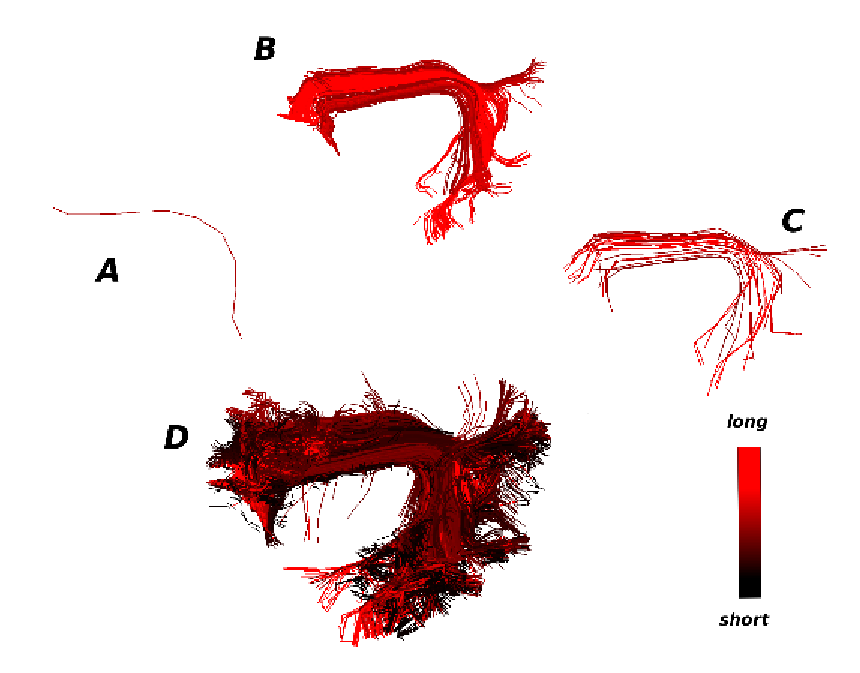
\includegraphics[scale=0.65]{Figures/Fig_10_arcuate_small_fibers}}
  \caption{What could be considered as the strength and limitation of QB
    is that short streamlines will be clustered differently than longer
    streamlines although they may belong in the same anatomical
    bundle. A solution to this problem is illustrated. The colormap here
    encodes streamline length. A: a single centroid streamline, B: the
    $245$ actual streamlines closer than $15$~mm (MDF distance), C: the
    streamlines from B clustered with $23$ centroid streamlines using QB
    with threshold $6.25$~mm, D: the $\num{3421}$ actual streamlines
    closer than $6$~mm ($\textrm{MAM}_{\textrm{min}}$ distance) from the
    centroid streamlines in C are shown. We can see that a great number
    of short streamlines have been brought together along with the
    streamlines in B. \label{Flo:arcuate_close}}
\end{figure}

Here we discuss two simple strategies for clustering short
streamlines. The first is an unsupervised technique and the second is
supervised.

1. Cluster the long streamlines using QB with distance threshold at
$10$~mm and then cluster the short streamlines (<$100$~mm) to a lower
threshold and assign them to their closest long streamline bundle from
the first clustering using the $\mathrm{MAM}_{\mathrm{min}}$ distance.

2. Read and cluster the tractography of a subject, pick a centroid
streamline and then find the closest streamlines to that selected
streamline using MDF, cluster the closest streamlines found from the
previous step and for each one of these new centroid streamlines find
the closest streamlines using the $\textrm{MAM}_{\textrm{min}}$
distance. We should now have an amalgamation of shorter and longer
streamlines in one cluster.

An example of this second strategy is shown in
Fig.~\ref{Flo:arcuate_close}. A single centroid streamline of interest
(A) from the region of arcuate fasciculus is selected
Fig.~\ref{Flo:arcuate_close}; the streamlines closer than 15~mm (MDF) to
the selected cluster are shown (B) and clustered with a distance
threshold of $6.25$~mm (C); finally from every centroid streamline in C
we find the closest streamlines (D) using the
$\textrm{MAM}_{\textrm{min}}$ distance from the entire tractography. In
this way we managed to bring together in a semi-automatic fashion an
entire bundle consisting both of long and short streamlines by just
selecting initially a single representative streamline.

\section{Discussion and conclusion}

We have presented a novel and powerful algorithm -- QuickBundles
(QB). This algorithm provides simplifications to the old problem of
revealing the detailed anatomy of the densely packed white matter which
has recently attracted much scientific attention; it can also be used
for any trajectory clustering problem and it is recommended when large
datasets are involved. QB can be used with all types of diffusion MRI
tractographies which generate streamlines (e.g. probabilistic or
deterministic) and it is independent of the reconstruction model. QB is
supported by a distance function MDF on the space of streamlines which
makes it a metric space. QB can achieve compression ratios of the order
of 200:1 depending on the distance threshold while preserving
characteristic information about the tractography.

In common with mainstream clustering algorithms such as k-means,
k-centers and expectation maximization, QB is not a global clustering
method therefore it can give different results under different initial
conditions of the dataset when there is no obvious distance threshold
which can separate the clusters into meaningful bundles; for example we
should expect different clusters under different permutations of the streamlines in a densely packed tractography. However, we found
that there is good agreement even between two clusterings of the same
tractography with different permutations. If the clusters are truly
separable by distances then there is a global solution independent of
permutations. This is often visible in smaller subsets of the initial
tractography. 

Other algorithms previously too slow to be used on the entire
tractography can now be used efficiently too if they start their clustering
on the output of QB rather than the initial full tractography.

We saw that QB is a linear time clustering method based on streamline
distances, which is on average linear time $\mathcal{O}(N)$ where $N$ is
the number of streamlines and with worst case $\mathcal{O}(N^{2})$ when
every streamline is a singleton cluster itself. Therefore QB is the
fastest known tractography clustering method and even real-time on
smaller tractographies ($\le$~\num{20000} streamlines, depending on
system CPU). We also showed that it uses a negligible amount of memory.

QB is fully automatic and very robust as when we use it we can find good
agreements even between different subjects. Additionally, it can be used
to explore multiple tractographies and find correspondences or
similarities between different tractographies. This can be facilitated
by the use of Bundle Adjacency (BA) a new similarity measure introduced
in this paper.

The reduction in dimensionality of the data achieved by QB means that
BOIs (bundles of interest) can be selected as an alternative to ROIs for
interrogating or labeling the datasets.  Our experience with ROI-based matter atlases (WMAs) is that they cannot
differentiate fibre directions i.e. several different bundles could cross an ROI. Therefore, ROIs constructed with a WMA
do not lead to anatomical bundles and typically lead to large sprawling sets of streamlines. BOIs seem to be a solution
to this problem and BOI creation can be facilitated by QB. Furthermore, we showed that QB can be used to find obscured
streamlines not visible to the user at first instance. Therefore, QB opens up the road to create rapid tools for exploring tractographies of any size.

In the future we would like to investigate different ways to merge QB
clusters by integrating prior information from neuroanatomists. We are
currently working on developing interactive tools which exploit the
simplification that QB provides \citep[see][]{GaryfallidisHBM2012}.

We have shown results with data from simulations, single and multiple
real subjects. The code for QuickBundles is freely available at
$\texttt{dipy.org}$.

\section*{Acknowledgements}
We gratefully acknowledge valuable discussions with Arno Klein and John
Griffiths on various aspects of this work.

\section*{Disclosure/Conflict-of-Interest Statement}
There are no conflicts of interest relating to this work.

\selectlanguage{british}%
\bibliographystyle{apalike2}
%\bibliographystyle{plainnat}
%\bibliographystyle{IEEEabrv, IEEEtran}
%\bibliographystyle{IEEEtran}
%\bibliographystyle{elsarticle-harv}
\selectlanguage{english}
\bibliography{diffusion}

\end{document}
